\chapter{Conjunto de Dados}

Neste trabalho foram utilizados dois conjuntos de dados compostos da sequência de aminoácidos de proteínas com estruturas resolvidas experimentalmente e da estrutura secundária atribuída aos seus resíduos por quatro diferentes algoritmos: DSSP \cite{Kabsch1983a}, Stride \cite{Frishman1995a}, Kaksi \cite{Martin2005b} e PROSS \cite{Srinivasan1999b}.

O primeiro conjunto selecionado é formado por  estruturas de alta qualidade e tem como finalidade ser utilizado na busca de regras de transição para o autômato celular capazes de reproduzir os padrões de estruturas secundárias presentes nas proteínas. Essas regras de transição são um dos elementos mais importantes desse trabalho, pois permitem avaliar a generalização do autômato celular, isto é, qual o grau de sucesso da aplicação do autômato celular para o universo de proteínas existentes.

O segundo conjunto selecionado é composto de quatro proteínas com altíssima identidade sequêncial, tendo no máximo 3 resíduos mutados entre as sequências de 56 aminoácidos, e diferentes estruturas terciárias e secundárias. 

%Esse conjunto foi selecionado por ser, possivelmente, o caso experimental mais desafiador para os métodos de predição de estrutura secundária. Como discutiremos ao longo do texto, todos os métodos de predição de estrutura secundária, assim como os de modelagem comparativa, tendem a falhar nesse conjunto devido à limitações teóricas dos métodos.

\section{Conjunto de dados de proteínas diversas para treinamento}

O conjunto de proteínas diversas utilizado para o treinamento do autômato celular foi obtido do banco de dados “Top8000” (versão de 2015). Esse banco de dados é organizado pelo Richardson Lab da Universidade de Duke (disponível em \href{https://github.com/rlabduke/reference_data}{github.com/rlabduke/reference\_data}). As estruturas de proteínas, separadas em cadeias quando há mais de uma por estrutura, atendem aos seguintes critérios:

\begin{itemize}
	\item{Resolução < 2.0 \AA}
	\item{MolProbity score < 2.0}
	\item{$\le 5 \%$ dos resíduos apresentando comprimentos de ligação anormais ( $> 4\sigma$)}
	\item{$\le 5 \%$ dos resíduos apresentando ângulos de ligação anormais ( $> 4\sigma$)}
	\item{$\le 5 \%$ dos resíduos com desvios anormais do  $C_\beta$ ( > 0.25 \AA)}
\end{itemize}

As proteínas selecionadas pelos critérios acima são subagrupadas de acordo com o grau de identidade sequencial: < 50\%, <70\% e <95\%.  Proteínas que apresentassem resíduos indeterminados na estrutura ou que tivessem algum erro durante a atribuição da estrutura secundária por algum dos quatro métodos foram removidos do conjunto. A tabela \ref{tab:top8000} mostra o número de cadeias utilizadas.
% PSLO Zé quantas proteínas foram perdidas por caus deste filtro? Vc não acha draástico demais?
% Zé - Vou verificar os números, mas acho q por volta de 5% foram removidas apenas. Não me parece um número ruim a ponto de comprometer o conjunto.

\begin{table}
    \myfloatalign
  \begin{tabularx}{\textwidth}{Xll} \toprule
    \tableheadline{Conjunto}   & \tableheadline{\# original}   & \tableheadline{\# utilizadas}  \\ 
    \midrule
    Top8000-hom50 & 7233 &  6749 \\
    Top8000-hom70 & 7958 & 7435 \\
    Top8000-hom95 & 8826 & 8227 \\
    %autem vulputate ex & parola & romanic \\
    %usu mucius iisque & studio & sanctificatef \\
    \bottomrule
  \end{tabularx}
  \caption{Número de cadeias presentes no banco de dados Top8000 (Richardson Lab) e número de cadeias utilizadas neste trabalho após a exclusão de cadeias que apresentaram algum problema durante a atribuição da estrutura secundária ou que possuiam resíduos indeterminados.}  \label{tab:top8000}
\end{table}

\section{Proteínas com altíssima identidade sequêncial e diferentes estruturas terciárias e secundárias}

Em 2007, Alexander e colaboradores \cite{Alexander2007}, desenharam um experimento onde obtiveram dois enovelamentos com topologias diferentes para sequências com mais de 88\% de identidade sequencial. O ponto de partida do experimento foram dois domínios chamados $G_A$ e $G_B$  com 56 aminoácidos.  O domínio $G_A$ possui um feixe de 3 hélices $\alpha$ (\textit{3-$\alpha$ helix bundle}) enquanto o domínio $G_B$ apresenta a enovelamento 4$\beta$+$\alpha$, ou seja, 4 fitas $\beta$ mais uma hélice $\alpha$ (Figura \ref{fig:ga_gb}).
% PSLO Zé esses domínios pertencem a qual proteína?

\begin{figure}
  \centering
  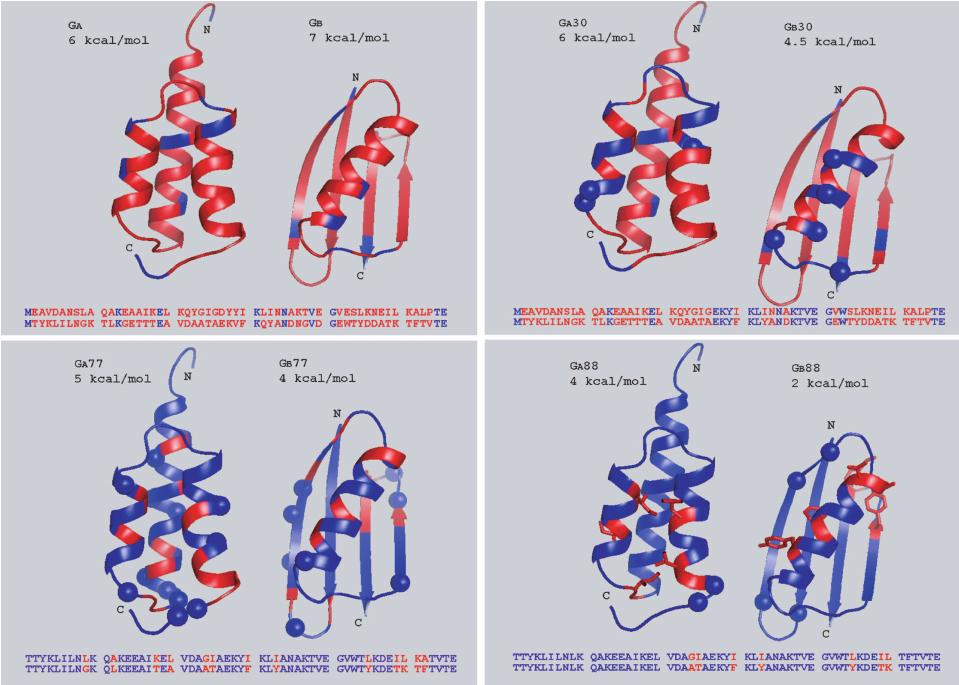
\includegraphics[width=1.0\textwidth]{figures/ga_gb.jpg}
  \caption{Figura representando o design dos domínios. Os resíduos em azul são as mutações introduzidas, esses resíduos são idênticos em ambas as sequências. Em vermelho estão os resíduos diferentes (Figura extraída de \cite{Alexander2007})}
        \label{fig:ga_gb}
\end{figure}

Posteriormente, uma série de outros estudos sobre esses dois domínios demonstrou ser possível obter os dois enovelamentos com idetidade sequencial ainda maiores \cite{He2008,Alexander2009}, até que em 2012, He e colaboradores \cite{He2012}, obtiveram mutações pontuais capazes de alterar a estrutura entre os dois enovelamentos (Figura \ref{fig:camaleonicas}). As estruturas resolvidas por RMN das quatro proteínas foram as utilizadas para compor esse conjunto de dados (PDB IDs: 2LHC, 2LHD, 2LHE, 2LHG) utilizando os 10 primeiros modelos de cada estruturas com o objetivo de manter os dados balanceados.

\begin{figure}
  \centering
  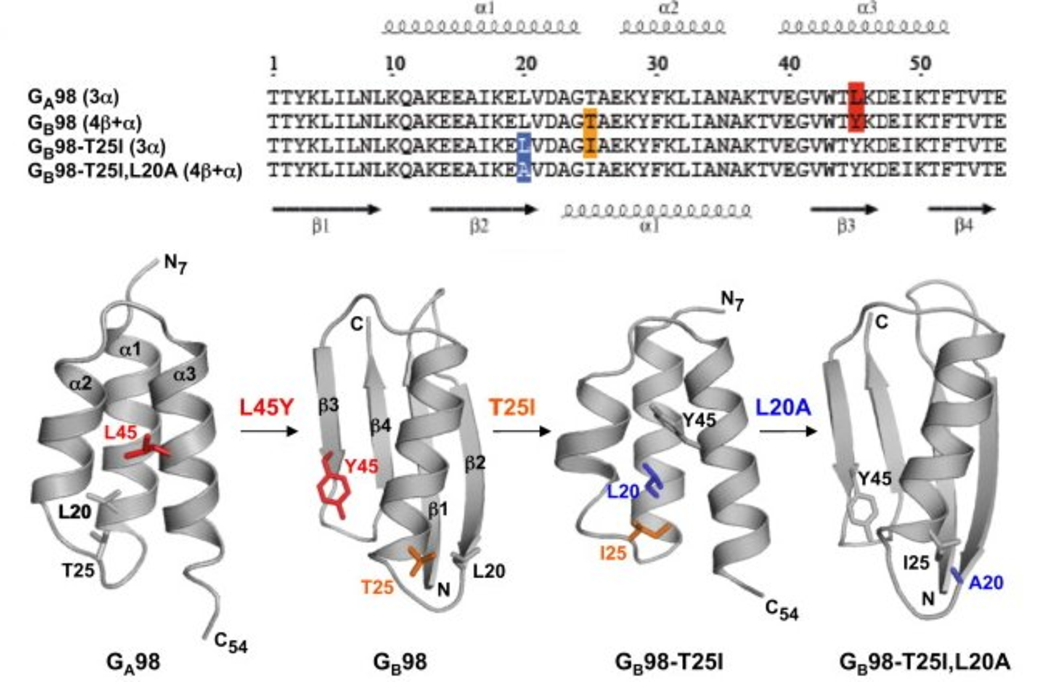
\includegraphics[width=1.0\textwidth]{figures/chameleonic_resume.pdf}
  \caption{Alinhamento das sequências de resíduos mostrando as mutaçoões que ocasionaram as mudanças entre as topologias $3\alpha$ e $4\alpha+\beta$ e os modelos estruturas indicando as posições das mutações (Figura adaptada de \cite{He2012})}
        \label{fig:camaleonicas}
\end{figure}
